\documentclass{beamer}
\usepackage[utf8]{inputenc}

\usetheme{Madrid}
\usecolortheme{default}
\usepackage{amsmath,amssymb,amsfonts,amsthm}
\usepackage{txfonts}
\usepackage{tkz-euclide}
\usepackage{listings}
\usepackage{adjustbox}
\usepackage{array}
\usepackage{tabularx}
\usepackage{gvv}
\usepackage{lmodern}
\usepackage{circuitikz}
\usepackage{tikz}
\usepackage{graphicx}

\setbeamertemplate{page number in head/foot}[totalframenumber]

\usepackage{tcolorbox}
\tcbuselibrary{minted,breakable,xparse,skins}

% Code styling
\lstset{
    language=C,
    basicstyle=\ttfamily\small,
    keywordstyle=\color{blue},
    stringstyle=\color{orange},
    commentstyle=\color{green!60!black},
    numbers=left,
    numberstyle=\tiny\color{gray},
    breaklines=true,
    showstringspaces=false,
}
%------------------------------------------------------------

\title
{1.11.10}
\date{September 14, 2025}
\author 
{AI25BTECH11008\\Chiruvella Harshith Sharan}

\begin{document}

\frame{\titlepage}

\begin{frame}{Question}
\centering
Find the direction cosines of the line joining points 
\[
P(4,3,-5) \quad \text{and} \quad Q(-2,1,8).
\]
\end{frame}


\begin{frame}{Theoretical Solution}
The points are $P(4,3,-5)$ and $Q(-2,1,8)$. \\[6pt]

$\vec{PQ} = \vec{Q} - \vec{P} 
= \myvec{-2-4 \\ 1-3 \\ 8-(-5)} 
= \myvec{-6 \\ -2 \\ 13}$ \\[10pt]

$|\vec{PQ}| = \sqrt{(-6)^2 + (-2)^2 + (13)^2} 
= \sqrt{36 + 4 + 169} 
= \sqrt{209}$ \\[6pt]

\[
\cos \alpha = \frac{-6}{\sqrt{209}}, \quad
\cos \beta = \frac{-2}{\sqrt{209}}, \quad
\cos \gamma = \frac{13}{\sqrt{209}}
\]

\begin{align}
\centering
\boxed{\text{Therefore, the direction cosines are } 
\left(\tfrac{-6}{\sqrt{209}}, \tfrac{-2}{\sqrt{209}}, \tfrac{13}{\sqrt{209}}\right).}
\end{align}
\end{frame}


% ------------------- C Code -------------------
\begin{frame}[fragile]
    \frametitle{C Code}
    \begin{lstlisting}
#include <stdio.h>
#include <math.h>

int main() {
    // Step 1: Define points P and Q
    double P[3] = {4, 3, -5};
    double Q[3] = {-2, 1, 8};

    // Step 2: Direction vector PQ = Q - P
    double PQ[3];
    PQ[0] = Q[0] - P[0];   // -6
    PQ[1] = Q[1] - P[1];   // -2
    PQ[2] = Q[2] - P[2];   // 13

    // Step 3: Magnitude of PQ
    double mag = sqrt(PQ[0]*PQ[0] + PQ[1]*PQ[1] + PQ[2]*PQ[2]);

    \end{lstlisting}
\end{frame}

\begin{frame}[fragile]
    \frametitle{Python Code}
    \begin{lstlisting}
    
    // Step 4: Direction cosines
    double cos_alpha = PQ[0] / mag;
    double cos_beta  = PQ[1] / mag;
    double cos_gamma = PQ[2] / mag;

    // Output
    printf("Vector PQ = (%.0f, %.0f, %.0f)\n", PQ[0], PQ[1], PQ[2]);
    printf("|PQ| = sqrt(209) = %.4f\n", mag);
    printf("Direction cosines:\n");
    printf("cos(alpha) = %.4f\n", cos_alpha);
    printf("cos(beta)  = %.4f\n", cos_beta);
    printf("cos(gamma) = %.4f\n", cos_gamma);

    return 0;
}

    \end{lstlisting}
\end{frame}

% ------------------- Python Plot -------------------
\begin{frame}[fragile]
    \frametitle{Python Code}
    \begin{lstlisting}
import numpy as np
import matplotlib.pyplot as plt
from mpl_toolkits.mplot3d import Axes3D

# Define the points
P = np.array([4, 3, -5])
Q = np.array([-2, 1, 8])

# Generate line PQ
t = np.linspace(0, 1, 100)
line = np.outer(1-t, P) + np.outer(t, Q)

# Plot
fig = plt.figure(figsize=(8, 6))
ax = fig.add_subplot(111, projection='3d')

# Plot line PQ
ax.plot(line[:, 0], line[:, 1], line[:, 2], 'b-', label='$PQ$')

    \end{lstlisting}
\end{frame}

\begin{frame}[fragile]
    \frametitle{Python Code}
    \begin{lstlisting}
    
# Plot points P and Q
ax.scatter(P[0], P[1], P[2], color='red', s=60, label='P(4,3,-5)')
ax.scatter(Q[0], Q[1], Q[2], color='green', s=60, label='Q(-2,1,8)')

# Annotate points
ax.text(P[0]+0.3, P[1]+0.3, P[2], 'P(4,3,-5)', fontsize=10, color='red')
ax.text(Q[0]+0.3, Q[1]+0.3, Q[2], 'Q(-2,1,8)', fontsize=10, color='green')

# Set labels
ax.set_xlabel('X-axis')
ax.set_ylabel('Y-axis')
ax.set_zlabel('Z-axis')

    \end{lstlisting}
\end{frame}

\begin{frame}[fragile]
    \frametitle{Python Code}
    \begin{lstlisting}
    
# Title
ax.set_title("Line joining P(4,3,-5) and Q(-2,1,8)")

# Grid and legend
ax.grid(True, linestyle='--', alpha=0.6)
ax.legend()

# Save and show
plt.savefig("fig1.png", dpi=300, bbox_inches="tight")
plt.show()

    \end{lstlisting}
\end{frame}

\begin{frame}{Plot}
   \centering
   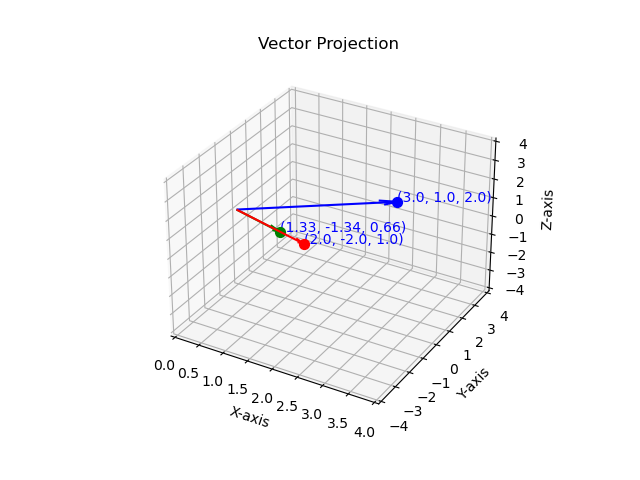
\includegraphics[width=\columnwidth, height=0.8\textheight, keepaspectratio]{figs/fig1.png}
   \label{fig:Beamer/figs/fig1.png}
\end{frame}

\end{document}
